

\tikzset{every picture/.style={line width=0.75pt}} %set default line width to 0.75pt        

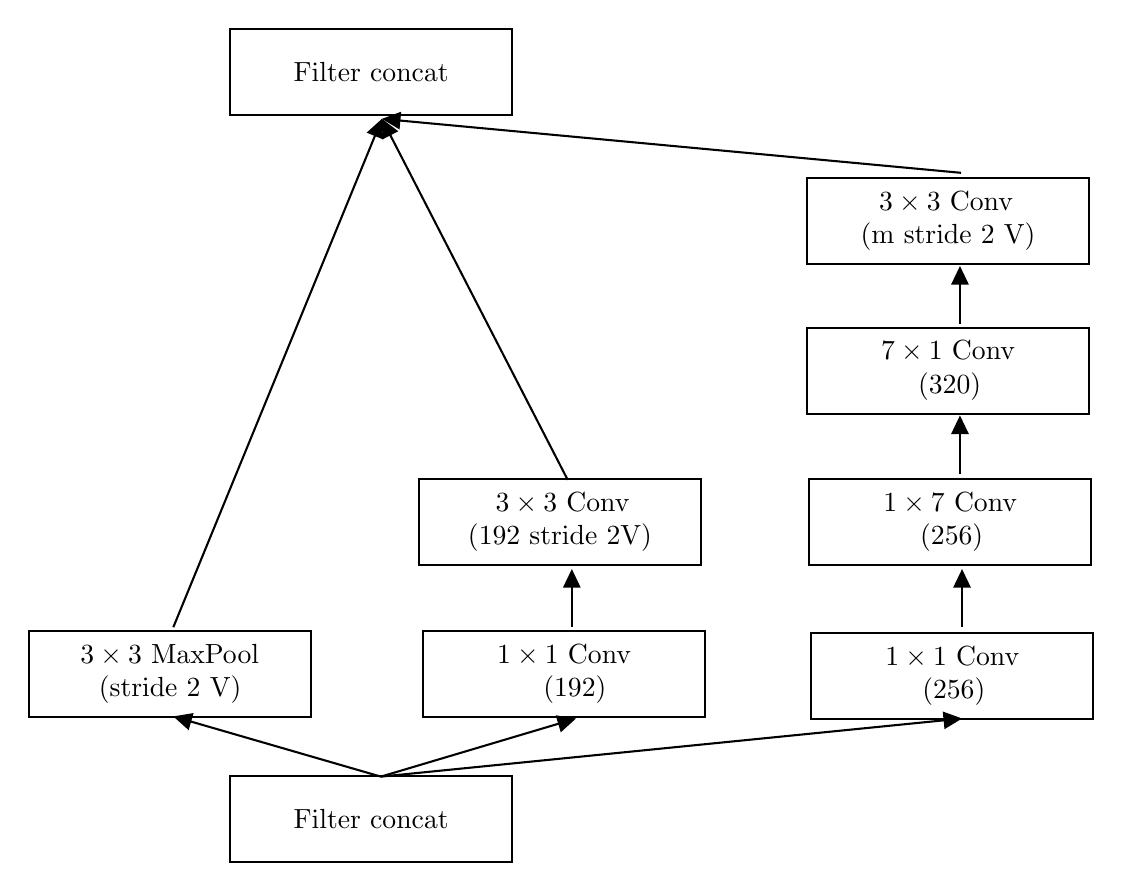
\begin{tikzpicture}[x=0.75pt,y=0.75pt,yscale=-1,xscale=1]
%uncomment if require: \path (0,470.3333282470703); %set diagram left start at 0, and has height of 470.3333282470703

%Flowchart: Process [id:dp24078826379297702] 
\draw   (528,418.9) -- (663.93,418.9) -- (663.93,460.33) -- (528,460.33) -- cycle ;
%Flowchart: Process [id:dp22165017848855517] 
\draw   (431,348.9) -- (566.93,348.9) -- (566.93,390.33) -- (431,390.33) -- cycle ;
%Flowchart: Process [id:dp6597264859137688] 
\draw   (621,348.9) -- (756.93,348.9) -- (756.93,390.33) -- (621,390.33) -- cycle ;
%Flowchart: Process [id:dp3799233367302206] 
\draw   (808,349.9) -- (943.93,349.9) -- (943.93,391.33) -- (808,391.33) -- cycle ;
%Straight Lines [id:da4490839848046586] 
\draw    (600.67,419.24) -- (502.59,390.8) ;
\draw [shift={(500.67,390.24)}, rotate = 376.16999999999996] [fill={rgb, 255:red, 0; green, 0; blue, 0 }  ][line width=0.75]  [draw opacity=0] (8.93,-4.29) -- (0,0) -- (8.93,4.29) -- cycle    ;

%Straight Lines [id:da38737183977033096] 
\draw    (600.67,419.24) -- (692.75,391.81) ;
\draw [shift={(694.67,391.24)}, rotate = 523.4100000000001] [fill={rgb, 255:red, 0; green, 0; blue, 0 }  ][line width=0.75]  [draw opacity=0] (8.93,-4.29) -- (0,0) -- (8.93,4.29) -- cycle    ;

%Straight Lines [id:da40057235552744497] 
\draw    (600.67,419.24) -- (878.68,391.44) ;
\draw [shift={(880.67,391.24)}, rotate = 534.29] [fill={rgb, 255:red, 0; green, 0; blue, 0 }  ][line width=0.75]  [draw opacity=0] (8.93,-4.29) -- (0,0) -- (8.93,4.29) -- cycle    ;

%Flowchart: Process [id:dp42511218119703864] 
\draw   (619,275.9) -- (754.93,275.9) -- (754.93,317.33) -- (619,317.33) -- cycle ;
%Flowchart: Process [id:dp6580432352234802] 
\draw   (807,275.9) -- (942.93,275.9) -- (942.93,317.33) -- (807,317.33) -- cycle ;
%Flowchart: Process [id:dp8669834254894924] 
\draw   (806,202.9) -- (941.93,202.9) -- (941.93,244.33) -- (806,244.33) -- cycle ;
%Straight Lines [id:da7396787751036953] 
\draw    (692.67,347.24) -- (692.67,321.24) ;
\draw [shift={(692.67,319.24)}, rotate = 450] [fill={rgb, 255:red, 0; green, 0; blue, 0 }  ][line width=0.75]  [draw opacity=0] (8.93,-4.29) -- (0,0) -- (8.93,4.29) -- cycle    ;

%Straight Lines [id:da2216611723462627] 
\draw    (880.67,347.24) -- (880.67,321.24) ;
\draw [shift={(880.67,319.24)}, rotate = 450] [fill={rgb, 255:red, 0; green, 0; blue, 0 }  ][line width=0.75]  [draw opacity=0] (8.93,-4.29) -- (0,0) -- (8.93,4.29) -- cycle    ;

%Straight Lines [id:da7609415385669374] 
\draw    (879.67,273.24) -- (879.67,247.24) ;
\draw [shift={(879.67,245.24)}, rotate = 450] [fill={rgb, 255:red, 0; green, 0; blue, 0 }  ][line width=0.75]  [draw opacity=0] (8.93,-4.29) -- (0,0) -- (8.93,4.29) -- cycle    ;

%Flowchart: Process [id:dp1491076780226832] 
\draw   (528,58.9) -- (663.93,58.9) -- (663.93,100.33) -- (528,100.33) -- cycle ;
%Straight Lines [id:da30781560796019103] 
\draw    (500.67,347.24) -- (600.41,104.18) ;
\draw [shift={(601.17,102.33)}, rotate = 472.31] [fill={rgb, 255:red, 0; green, 0; blue, 0 }  ][line width=0.75]  [draw opacity=0] (8.93,-4.29) -- (0,0) -- (8.93,4.29) -- cycle    ;

%Straight Lines [id:da24908463720618457] 
\draw    (690.67,276.24) -- (602.08,104.11) ;
\draw [shift={(601.17,102.33)}, rotate = 422.77] [fill={rgb, 255:red, 0; green, 0; blue, 0 }  ][line width=0.75]  [draw opacity=0] (8.93,-4.29) -- (0,0) -- (8.93,4.29) -- cycle    ;

%Flowchart: Process [id:dp01199680277761872] 
\draw   (806,130.9) -- (941.93,130.9) -- (941.93,172.33) -- (806,172.33) -- cycle ;
%Straight Lines [id:da3952124421996095] 
\draw    (879.67,201.24) -- (879.67,175.24) ;
\draw [shift={(879.67,173.24)}, rotate = 450] [fill={rgb, 255:red, 0; green, 0; blue, 0 }  ][line width=0.75]  [draw opacity=0] (8.93,-4.29) -- (0,0) -- (8.93,4.29) -- cycle    ;

%Straight Lines [id:da25220885973901197] 
\draw    (880.17,128.33) -- (603.16,102.52) ;
\draw [shift={(601.17,102.33)}, rotate = 365.32] [fill={rgb, 255:red, 0; green, 0; blue, 0 }  ][line width=0.75]  [draw opacity=0] (8.93,-4.29) -- (0,0) -- (8.93,4.29) -- cycle    ;


% Text Node
\draw (595.96,439.62) node  [align=left] {Filter concat};
% Text Node
\draw (498.96,369.62) node  [align=left] {$\displaystyle 3\times 3$ MaxPool\\ \ \ (stride $\displaystyle 2$ V)};
% Text Node
\draw (688.96,369.62) node  [align=left] {$\displaystyle 1\times 1$ Conv\\ \ \ \ \ \ ($\displaystyle 192$)};
% Text Node
\draw (875.96,370.62) node  [align=left] {$\displaystyle 1\times 1$ Conv\\ \ \ \ \ ($\displaystyle 256$)};
% Text Node
\draw (686.96,296.62) node  [align=left] {$\displaystyle \ \ \ 3\times 3$ Conv\\($\displaystyle 192$ stride $\displaystyle 2$V)};
% Text Node
\draw (874.96,296.62) node  [align=left] {$\displaystyle 1\times 7$ Conv\\ \ \ \ \ ($\displaystyle 256$)};
% Text Node
\draw (873.96,223.62) node  [align=left] {$\displaystyle 7\times 1$ Conv\\ \ \ \ \ ($\displaystyle 320$)};
% Text Node
\draw (595.96,79.62) node  [align=left] {Filter concat};
% Text Node
\draw (873.96,151.62) node  [align=left] {$\displaystyle \ \ 3\times 3$ Conv\\(m stride $\displaystyle 2$ V)};


\end{tikzpicture}